% This file was created by tikzplotlib v0.9.6.
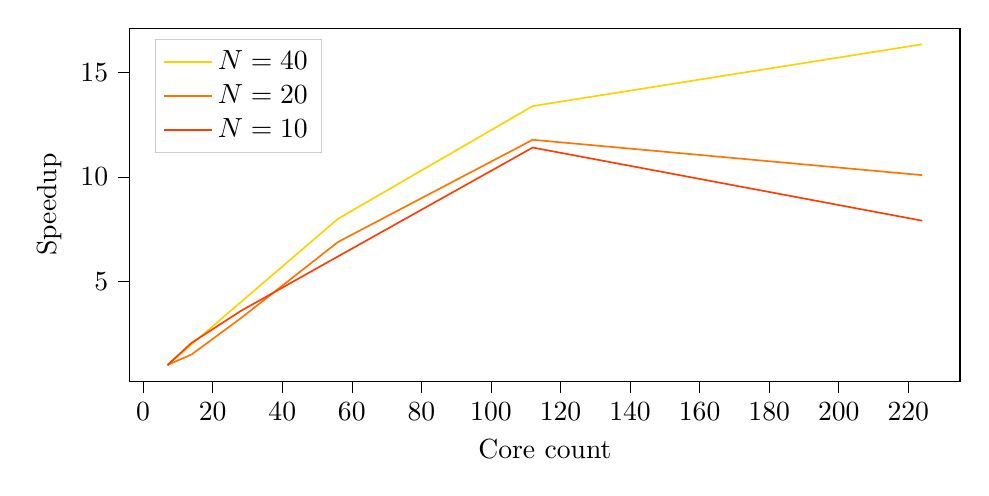
\begin{tikzpicture}

\definecolor{color0}{rgb}{1,0.81999231064975,0}
\definecolor{color1}{rgb}{1,0.456286043829296,0}
\definecolor{color2}{rgb}{1,0.238062283737024,0}

\begin{axis}[
height=0.5\textwidth,
legend cell align={left},
legend style={fill opacity=0.8, draw opacity=1, text opacity=1, at={(0.03,0.97)}, anchor=north west, draw=white!80!black},
tick align=outside,
tick pos=left,
width=\textwidth,
x grid style={white!69.0196078431373!black},
xlabel={Core count},
xmin=-3.85, xmax=234.85,
xtick style={color=black},
y grid style={white!69.0196078431373!black},
ylabel={Speedup},
ymin=0.232060727093392, ymax=17.1267247310388,
ytick style={color=black}
]
\addplot [semithick, color0]
table {%
7 1
14 2
28 4
56 8
112 13.3986405956246
224 16.3587854581322
};
\addlegendentry{$N = 40$}
\addplot [semithick, color1]
table {%
7 1
14 1.51423239878248
28 3.22970269035864
56 6.88864405993413
112 11.7860629390055
224 10.091984097319
};
\addlegendentry{$N = 20$}
\addplot [semithick, color2]
table {%
7 1
14 2.07015925720962
28 3.5819768060432
56 6.19790132547864
112 11.4125423728814
224 7.91047932330827
};
\addlegendentry{$N = 10$}
\end{axis}

\end{tikzpicture}
